% =================================================================================================
% File:			client_tier/model.tex
% Description:	Defiinisce la sezione relativa al front-end dell'applicazione
% Created:		2015-04-07
% Author:		Tesser Paolo
% Email:		tesser.paolo@mashup-unipd.it
% =================================================================================================
% Modification History:
% Version		Modifier Date		Change											Author
% 0.0.1 		2015-04-07 			creato scheletro								Tesser Paolo
% =================================================================================================
%
%

% CONTENUTO DEL CAPITOLO


\subsubsection{bdsm\_app::client::model} % (fold)
\label{ssub:bdsm_app_client_model}
\begin{figure}[htbp]
	\centering
	\centerline{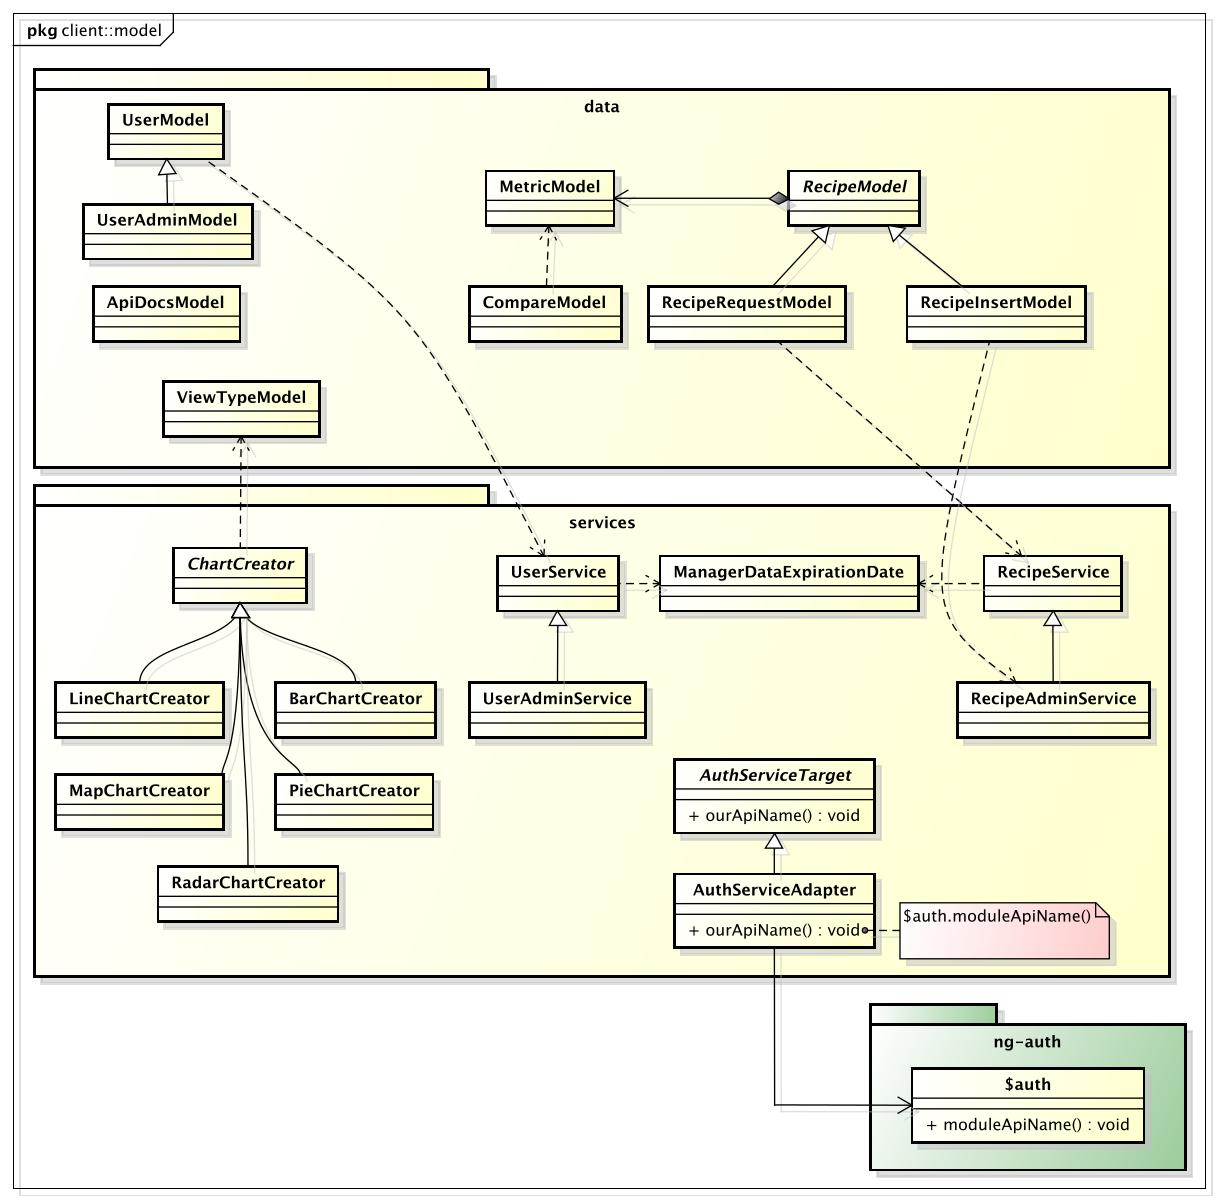
\includegraphics[scale=1.02]{./images/client/client_model.pdf}}
	\caption{Package - client::model}
\end{figure}

\begin{itemize}
	\item \textbf{Descrizione}: è il package che contiene sia le classi dei modelli di dati utilizzati dal client sia i servizi che mettono in comunicazione esso con il server attraverso i diversi servizi REST;
	\item \textbf{Padre}: client;
	\item \textbf{Package contenuti}:
		\begin{itemize}
			\item client::model::data
			\item client::model::services
		\end{itemize}
	\item \textbf{Interazione con altri componenti}:
		\begin{itemize}
			\item client::controller
		\end{itemize}
\end{itemize}
% subsubsection bdsm_app_client_model (end)

% PACKAGE MODEL::DATA
% =================================================================================================
% File:			client_tier/model/data.tex
% Description:	Defiinisce la sezione relativa al front-end dell'applicazione
% Created:		2015-04-10
% Author:		Tesser Paolo
% Email:		tesser.paolo@mashup-unipd.it
% =================================================================================================
% Modification History:
% Version		Modifier Date		Change											Author
% 0.0.1 		2015-04-10 			creato scheletro								Tesser Paolo
% =================================================================================================
%
%

% CONTENUTO DEL CAPITOLO
%

\subsubsection{bdsm\_app::client::model::data} % (fold)
\label{ssub:bdsm_app_client_model_data}
[TO DO] (diagramma) \newline \newline

\begin{itemize}
	\item \textbf{Descrizione}: [TO DO];
	\item \textbf{Padre}: client::model
	\item \textbf{Interazione con altri componenti}:
		\begin{itemize}
			\item client::model::services
			\item client::controller
		\end{itemize}

	\paragraph{Classi} % (fold)
		\subparagraph{Nome package::Nome classe} % (fold)
		\label{subp:subparagraph_name}
			\begin{itemize}
				\item \textbf{Descrizione}: [TO DO];
				\item \textbf{Utilizzo}: [TO DO];
				\item \textbf{Classi ereditate}: [TO DO];
				\item \textbf{Relazioni con altre classi}: [TO DO].
			\end{itemize}
\end{itemize}
% subsubsection bdsm_app_client_model_data (end) % \clearpage \newpage
% END PACKAGE MODEL::DATA

% PACKAGE MODEL::SERVICES
% =================================================================================================
% File:			client_tier/model/services.tex
% Description:	Defiinisce la sezione relativa al front-end dell'applicazione
% Created:		2015-04-10
% Author:		Tesser Paolo
% Email:		tesser.paolo@mashup-unipd.it
% =================================================================================================
% Modification History:
% Version		Modifier Date		Change											Author
% 0.0.1 		2015-04-10 			creato scheletro								Tesser Paolo
% =================================================================================================
%
%

% CONTENUTO DEL CAPITOLO
%

\subsubsection{bdsm\_app::client::model::services} % (fold)
\label{ssub:bdsm_app_client_model_services}
[TO DO] (diagramma) \newline \newline

\begin{itemize}
	\item \textbf{Descrizione}: [TO DO];
	\item \textbf{Padre}: client::model
	\item \textbf{Interazione con altri componenti}:
		\begin{itemize}
			\item client::model::data
			\item client::controller
		\end{itemize}
	
	\paragraph{Classi} % (fold)

		\subparagraph{client::model::services::AuthService} % (fold)
		\label{subp:client_model_services_authservice}
			\begin{itemize}
				\item \textbf{Descrizione}: [TO DO];
				\item \textbf{Utilizzo}: [TO DO];
				\item \textbf{Classi ereditate}: [TO DO];
				\item \textbf{Relazioni con altre classi}: [TO DO].
			\end{itemize}
		
		\subparagraph{client::model::services::RecipeService} % (fold)
		\label{subp:client_model_services_recipeservice}
			\begin{itemize}
				\item \textbf{Descrizione}: [TO DO];
				\item \textbf{Utilizzo}: [TO DO];
				\item \textbf{Classi ereditate}: [TO DO];
				\item \textbf{Relazioni con altre classi}: [TO DO].
			\end{itemize}
		% subparagraph client_model_services_recipeservice (end)

		\subparagraph{client::model::services::RecipeAdminService} % (fold)
		\label{subp:client_model_services_recipeadminservice}
			\begin{itemize}
				\item \textbf{Descrizione}: [TO DO];
				\item \textbf{Utilizzo}: [TO DO];
				\item \textbf{Classi ereditate}: [TO DO];
				\item \textbf{Relazioni con altre classi}: [TO DO].
			\end{itemize}
		% subparagraph client_model_services_recipeadminservice (end)


		\subparagraph{client::model::services::UserService} % (fold)
		\label{subp:client_model_services_userservice}
			\begin{itemize}
				\item \textbf{Descrizione}: [TO DO];
				\item \textbf{Utilizzo}: [TO DO];
				\item \textbf{Classi ereditate}: [TO DO];
				\item \textbf{Relazioni con altre classi}: [TO DO].
			\end{itemize}
		% subparagraph client_model_services_userservice (end)

		\subparagraph{client::model::services::UserAdminService} % (fold)
		\label{subp:client_model_services_useradminservice}
			\begin{itemize}
				\item \textbf{Descrizione}: [TO DO];
				\item \textbf{Utilizzo}: [TO DO];
				\item \textbf{Classi ereditate}: [TO DO];
				\item \textbf{Relazioni con altre classi}: [TO DO].
			\end{itemize}
		% subparagraph client_model_services_useradminservice (end)

		\subparagraph{ChartCreator} % (fold)
		\label{subp:chartcreator}
			\begin{itemize}
				\item \textbf{Descrizione}: [TO DO];
				\item \textbf{Utilizzo}: [TO DO];
				\item \textbf{Classi ereditate}: [TO DO];
				\item \textbf{Relazioni con altre classi}: [TO DO].
			\end{itemize}
		% subparagraph chartcreator (end)

		\subparagraph{LineChartCreator} % (fold)
		\label{subp:linechartcreator}
			\begin{itemize}
				\item \textbf{Descrizione}: [TO DO];
				\item \textbf{Utilizzo}: [TO DO];
				\item \textbf{Classi ereditate}: [TO DO];
				\item \textbf{Relazioni con altre classi}: [TO DO].
			\end{itemize}
		% subparagraph linechartcreator (end)


		\subparagraph{BarChartCreator} % (fold)
		\label{subp:barchartcreator}
			\begin{itemize}
				\item \textbf{Descrizione}: [TO DO];
				\item \textbf{Utilizzo}: [TO DO];
				\item \textbf{Classi ereditate}: [TO DO];
				\item \textbf{Relazioni con altre classi}: [TO DO].
			\end{itemize}
		% subparagraph barchartcreator (end)

		\subparagraph{PieChartCreator} % (fold)
		\label{subp:piechartcreator}
			\begin{itemize}
				\item \textbf{Descrizione}: [TO DO];
				\item \textbf{Utilizzo}: [TO DO];
				\item \textbf{Classi ereditate}: [TO DO];
				\item \textbf{Relazioni con altre classi}: [TO DO].
			\end{itemize}
		% subparagraph piechartcreator (end)

		\subparagraph{MapChartCreator} % (fold)
		\label{subp:mapchartcreator}
			\begin{itemize}
				\item \textbf{Descrizione}: [TO DO];
				\item \textbf{Utilizzo}: [TO DO];
				\item \textbf{Classi ereditate}: [TO DO];
				\item \textbf{Relazioni con altre classi}: [TO DO].
			\end{itemize}
		% subparagraph mapchartcreator (end)



\end{itemize}
% subsubsection bdsm_app_client_model_services (end)
% END PACKAGE MODEL::SERVICES
